
\subsection{Detailed analysis of \texttt{SOMVAEprob} patient states}
\label{subsec:detailed_icu}

As mentioned in the main text (see Fig \ref{fig:ICU_representations}) the \texttt{SOMVAEProb}
is able to uncover compact and interpretable structures in the latent space with respect
to future physiology scores. In this section we show results for acute physiology scores
in greater detail, analyze enrichment for future mortality risk, arguably the most
important severity indicator in the ICU, and explore phenotypes for particular 
physiological abnormalities.

% Acute physiology scores

\subsubsection*{Full results for future acute physiology scores}

\begin{figure}[h!]

\centering
\begin{subfigure}[t]{0.30\textwidth}
\centering
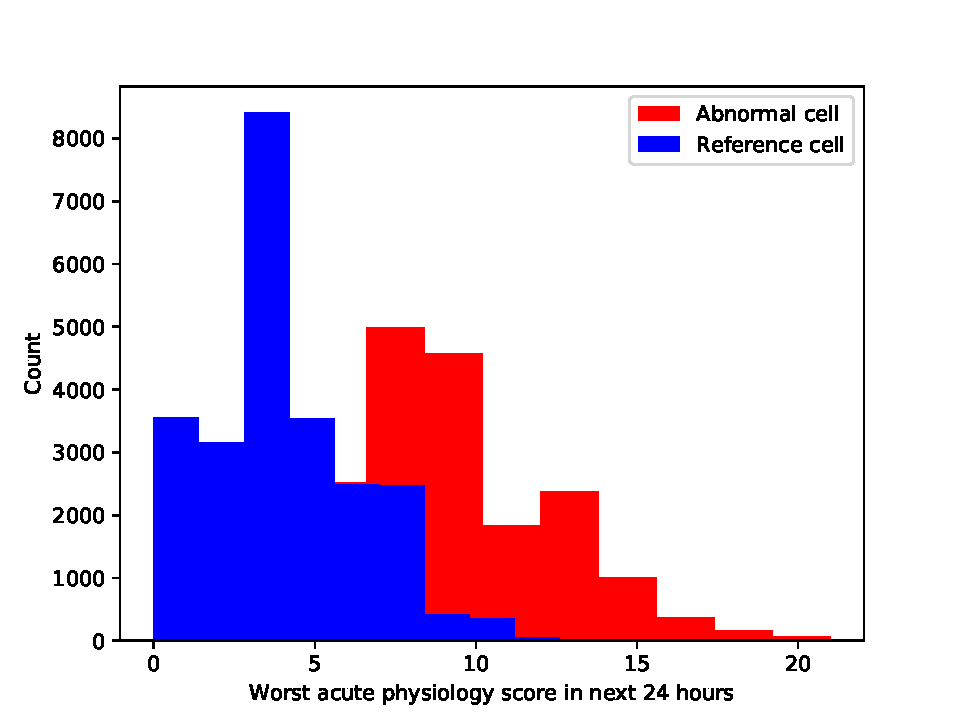
\includegraphics[scale=0.30]{./figures/icu_somvaeprob/distribution_cells}
\caption{Abnormal vs. reference cell}
\end{subfigure}
\begin{subfigure}[t]{0.30\textwidth}
\centering
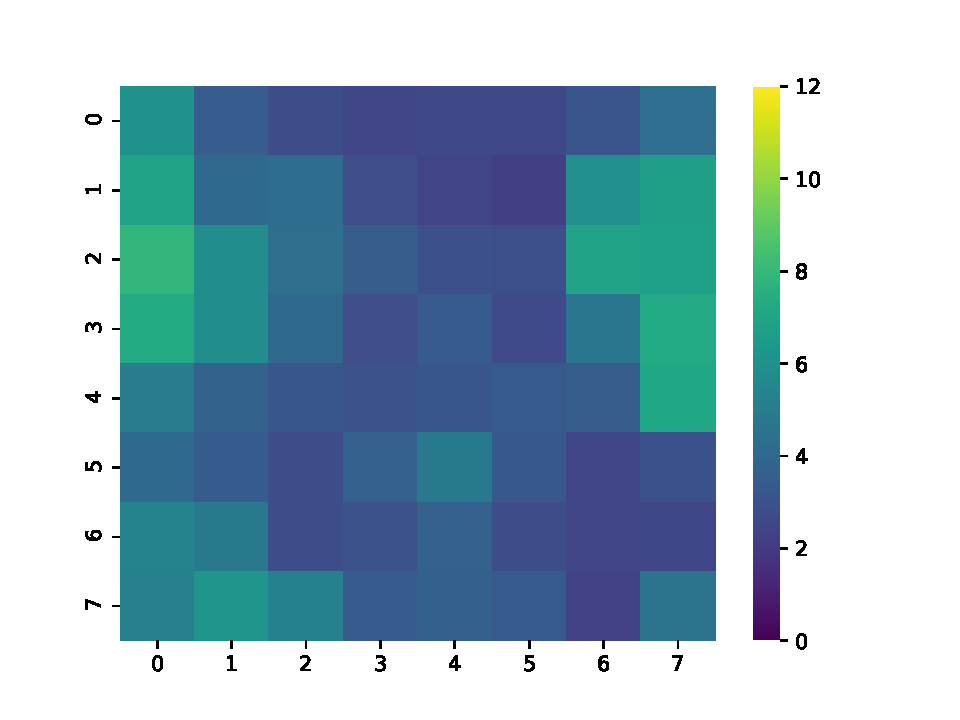
\includegraphics[scale=0.30]{./figures/icu_somvaeprob/detail_heatmaps_full_score_6}
\caption{Acute physiology score (6)}
\end{subfigure}
\begin{subfigure}[t]{0.30\textwidth}
\centering
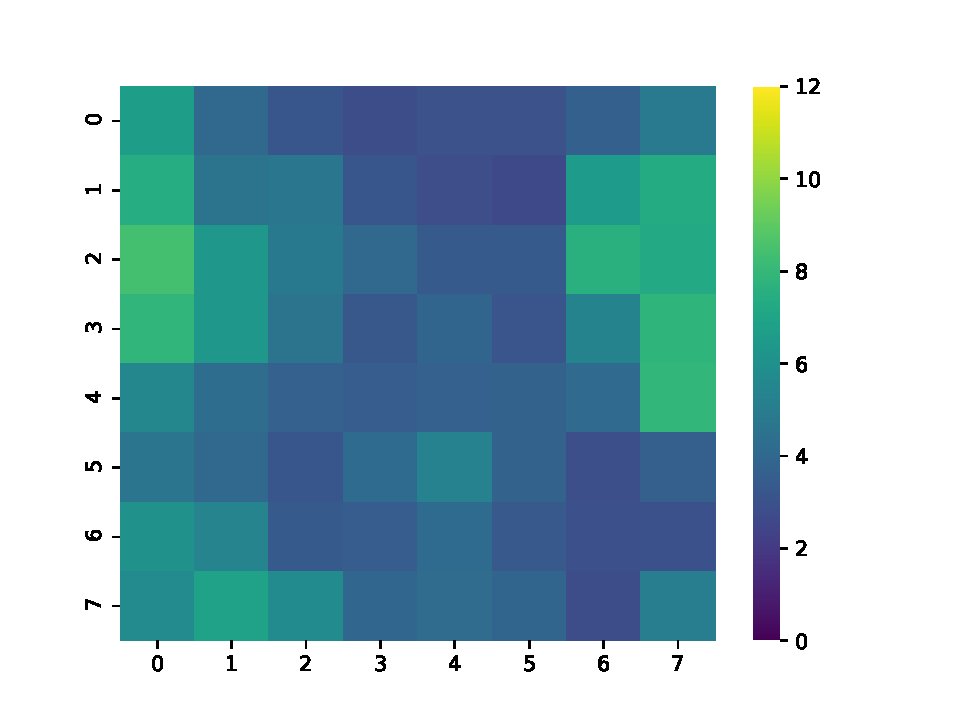
\includegraphics[scale=0.30]{./figures/icu_somvaeprob/detail_heatmaps_full_score_12}
\caption{ Acute physiology score (12)}
\end{subfigure}

\caption{(a) shows the difference in distribution of the acute
         physiology score in the next 24 hours, between time-points assigned to the most 
         abnormal cell in the \texttt{SOMVAEprob} map with coordinates [2,0] vs. 
         a normal cell chosen from the middle of the map with coordinates [4,3]. It is apparent that
         the distributions are largely disjoint, which means that the representation induced by 
         \texttt{SOMVAEprob} clearly distinguishes these risk profiles. Statistical tests for difference
         in distribution and location parameter are highly significant at p-values of $p \leq 10^{-3}$, as we
         have validated using a 2-sample $t$-test and Kolmogorov-Smirnov test. In (b-c) the enrichment 
         of the map for the mean acute physiology score in the next 6 and 12 hours is shown, for completeness.
         The enrichment patterns on the 3 maps, for the future horizons $\{6,12,24\}$, are almost identical, 
         which provides empirical evidence for the temporal stability of the \texttt{SOMVAEProb} embedding.}

\end{figure}

% Dynamic mortality in the next {12,24} hours

\subsubsection*{Dynamic mortality risk of patients on the \texttt{SOMVAEprob} map}

\begin{figure}[h!]
\centering
\begin{subfigure}[t]{0.47\textwidth}
\centering
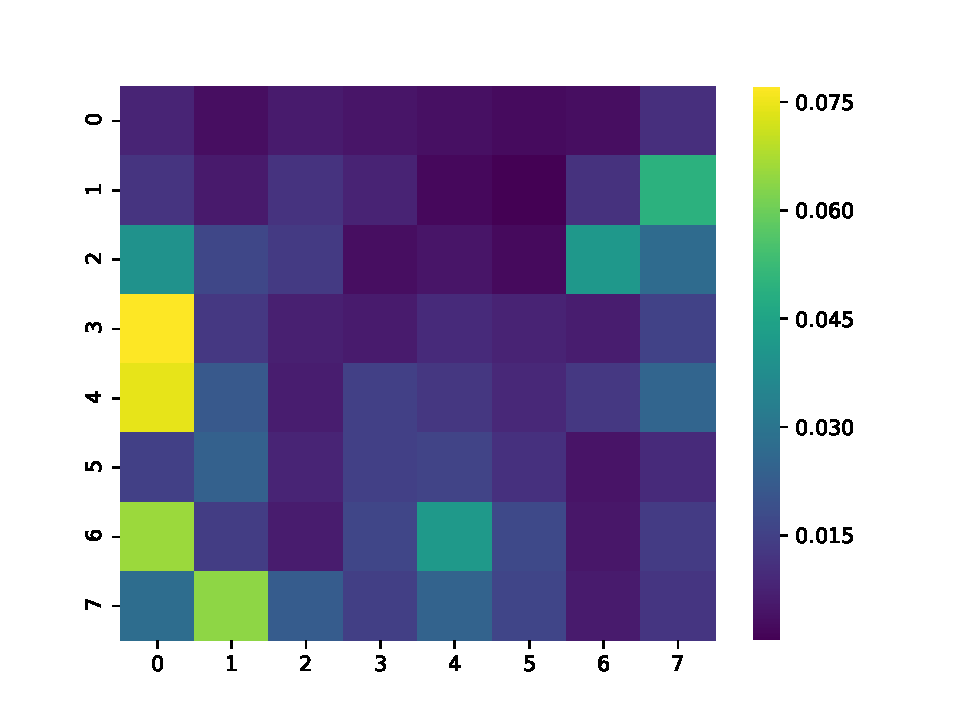
\includegraphics[scale=0.4]{./figures/icu_somvaeprob/detail_heatmaps_unit_discharge_expired_24}
\caption{24-hour mortality risk}
\end{subfigure}
\begin{subfigure}[t]{0.47\textwidth}
\centering
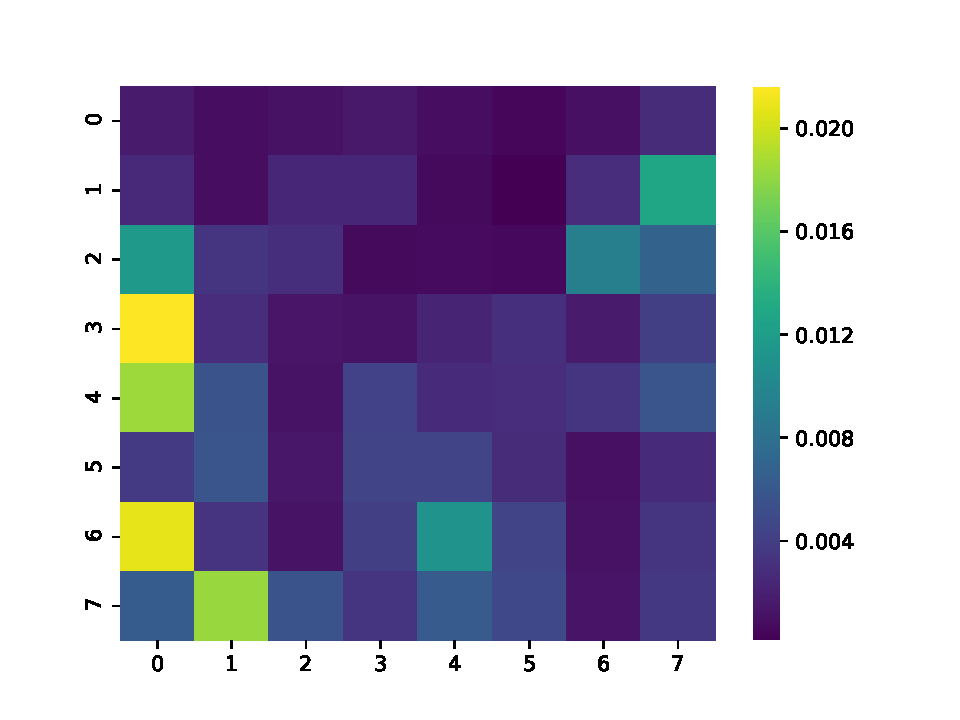
\includegraphics[scale=0.4]{./figures/icu_somvaeprob/detail_heatmaps_unit_discharge_expired_6}
\caption{6-hour mortality risk}
\end{subfigure}
\caption{(a) Dynamic mortality risk in the next 24 hours. (b) Short-term dynamic mortality risk in the next
             6 hours. We observe that the left-edge and right-edge regions of the \texttt{SOMVAEprob} map which
             are enriched for higher acute physiology scores (see Fig \ref{fig:ICU_representations}) also exhibit elevated 
             mortality rates over the baseline. Interestingly, according to future mortality risk, which is an important severity indicator,
             patients on the left-edge are significantly more sick on average than those on the right edge, which is
             less visible from the enrichment for acute physiology scores.}
\end{figure}

\newpage

% Detailed analysis of vital sign abnormalities

\subsubsection*{Patient state phenotypes on the \texttt{SOMVAEprob} map}

\begin{figure}[h!]
\centering
\begin{subfigure}[t]{0.22\textwidth}
\centering
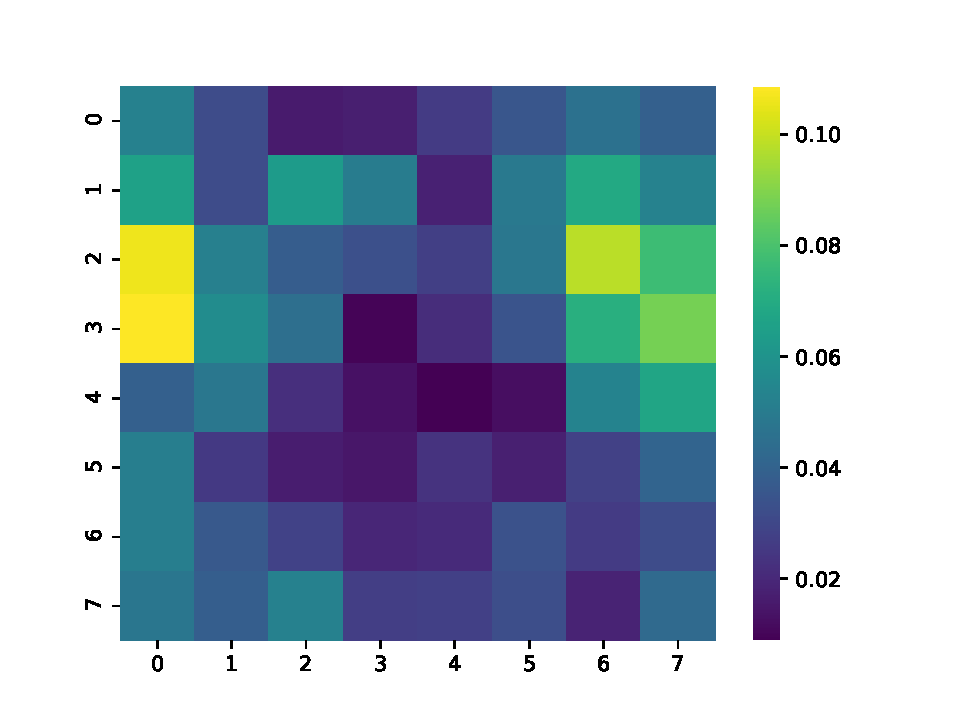
\includegraphics[scale=0.22]{./figures/icu_somvaeprob/detail_heatmaps_low_sodium}
\caption{Low Sodium}
\end{subfigure}
\begin{subfigure}[t]{0.22\textwidth}
\centering
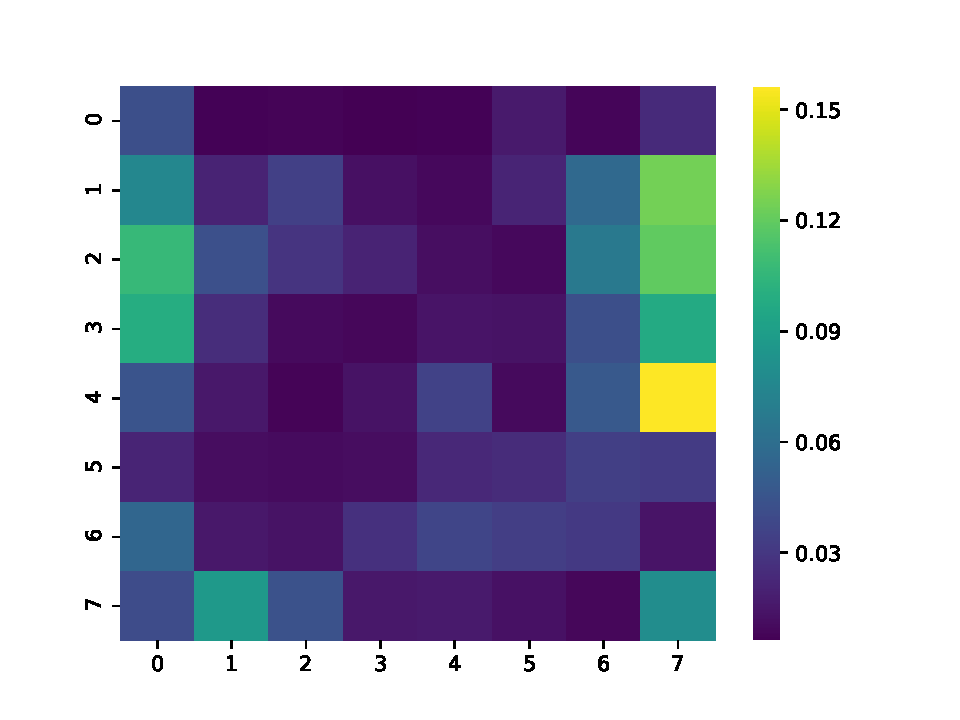
\includegraphics[scale=0.22]{./figures/icu_somvaeprob/detail_heatmaps_high_potassium}
\caption{High Potassium}
\end{subfigure}
\begin{subfigure}[t]{0.22\textwidth}
\centering
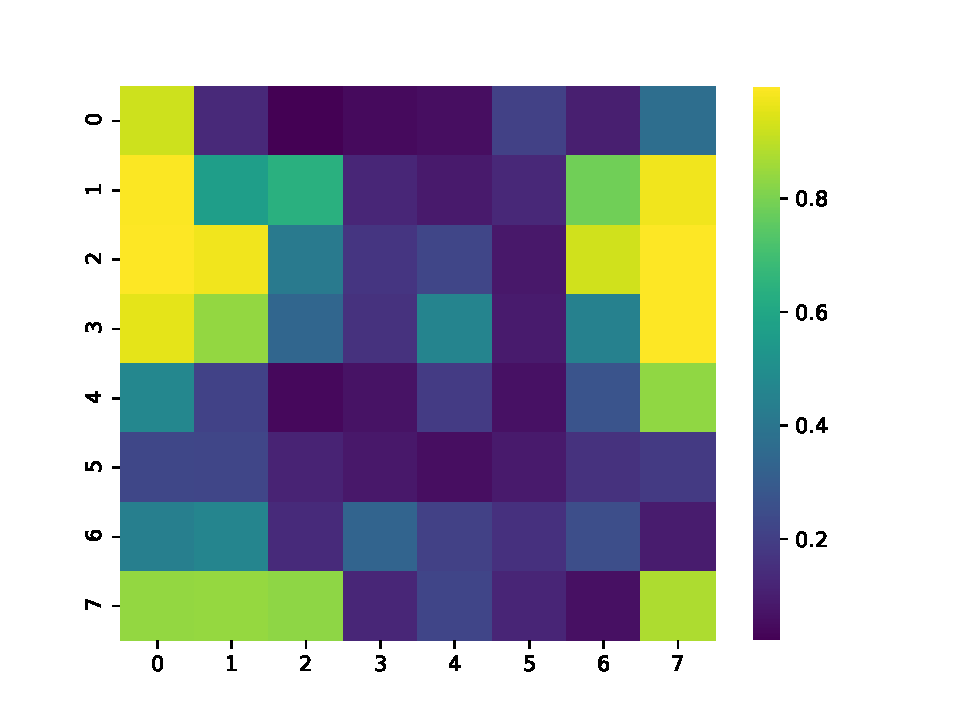
\includegraphics[scale=0.22]{./figures/icu_somvaeprob/detail_heatmaps_high_creatinine}
\caption{High Creatinine}
\end{subfigure}
\begin{subfigure}[t]{0.22\textwidth}
\centering
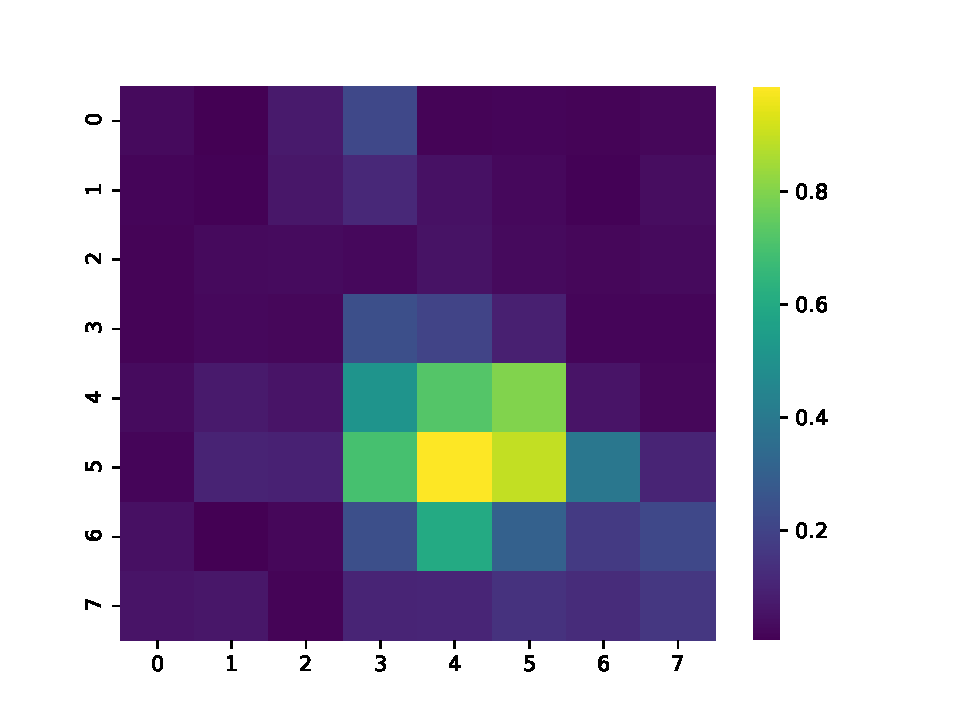
\includegraphics[scale=0.22]{./figures/icu_somvaeprob/detail_heatmaps_high_hco3}
\caption{High HCO3}
\end{subfigure}



\caption{(a) Prevalence of abnormally low sodium lab value in the next 24 
         hours, (b-d) Prevalence of abnormally high potassium/creatinine/HCO3 lab values in the next 24 hours. Each
         sub-figure illustrates the enrichment of a distinct phenotype on the \texttt{SOMVAEprob} map. Low sodium
         and high potassium states are enriched near the left edge, and near the right edge, respectively, which could
         represent sub-types of the high-risk phenotype found in these regions (compare Fig \ref{fig:ICU_representations}
         for the distribution of the acute physiology score). Elevated creatinine is a trait that occurs in both these regions.
         A compact structure associated with elevated HCO3 can be found in the center of the map, which could represent 
         a distinct phenotype with lower mortality risk in our cohort. In all phenotypes, the tendency of \texttt{SOMVAEprob}
         to recover compact structures is exemplified.}
\end{figure}
